\textbf{\LARGE{\color{tumgadPurple}Binary Heaps}}\\
\\
\noindent
Given the following \href{https://ossner.github.io/TUMGAD/src/DataStructures/PriorityQueues/BinaryHeaps/BinaryHeaps}{\underline{Binary $MINMAX$Heap}}:
%$INITTREE$
a) Perform the following insert-operations and their corresponding sift-operations on the above heap:
\begin{center}
    $INSERTIONS$
\end{center}
Insert: \underline{\hspace{.8cm}}
\begin{center}
    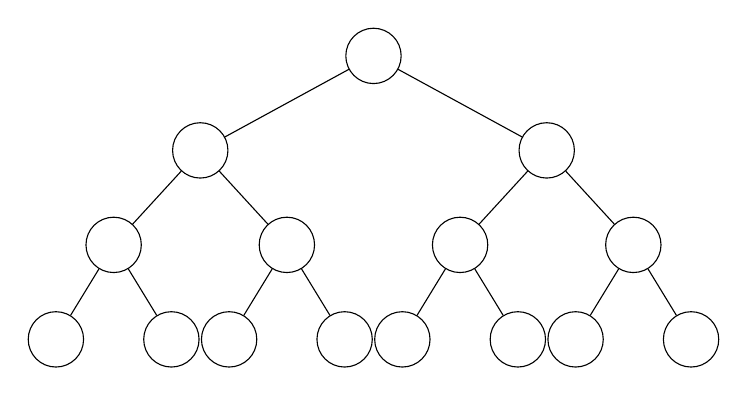
\begin{tikzpicture}[level/.style={sibling distance=55mm/#1},minimum size=25pt,scale=0.8,
        every node/.style={transform shape}]
        \node[circle,draw](z){}
        child{node[circle,draw]{}
            child{node[circle,draw]{}
                child{node[circle,draw]{}
                    child[missing]{}
                    child[missing]{}}
                child{node[circle,draw]{}
                    child[missing]{}
                    child[missing]{}}}
            child{node[circle,draw]{}
                child{node[circle,draw]{}
                    child[missing]{}
                    child[missing]{}}
                child{node[circle,draw]{}
                    child[missing]{}
                    child[missing]{}}}}
        child{node[circle,draw]{}
            child{node[circle,draw]{}
                child{node[circle,draw]{}
                    child[missing]{}
                    child[missing]{}}
                child{node[circle,draw]{}
                    child[missing]{}
                    child[missing]{}}}
            child{node[circle,draw]{}
                child{node[circle,draw]{}
                    child[missing]{}
                    child[missing]{}}
                child{node[circle,draw]{}
                    child[missing]{}
                    child[missing]{}}}};
    \end{tikzpicture}
\end{center}
Insert: \underline{\hspace{.8cm}}
\begin{center}
    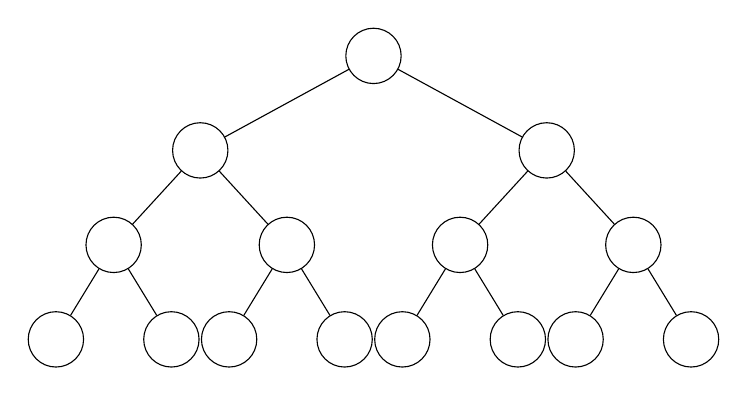
\begin{tikzpicture}[level/.style={sibling distance=55mm/#1},minimum size=25pt,scale=0.8,
    every node/.style={transform shape}]
        \node[circle,draw](z){}
        child{node[circle,draw]{}
            child{node[circle,draw]{}
                child{node[circle,draw]{}
                    child[missing]{}
                    child[missing]{}}
                child{node[circle,draw]{}
                    child[missing]{}
                    child[missing]{}}}
            child{node[circle,draw]{}
                child{node[circle,draw]{}
                    child[missing]{}
                    child[missing]{}}
                child{node[circle,draw]{}
                    child[missing]{}
                    child[missing]{}}}}
        child{node[circle,draw]{}
            child{node[circle,draw]{}
                child{node[circle,draw]{}
                    child[missing]{}
                    child[missing]{}}
                child{node[circle,draw]{}
                    child[missing]{}
                    child[missing]{}}}
            child{node[circle,draw]{}
                child{node[circle,draw]{}
                    child[missing]{}
                    child[missing]{}}
                child{node[circle,draw]{}
                    child[missing]{}
                    child[missing]{}}}};
    \end{tikzpicture}
\end{center}
\newpage
\noindent
Insert: \underline{\hspace{.8cm}}
\begin{center}
    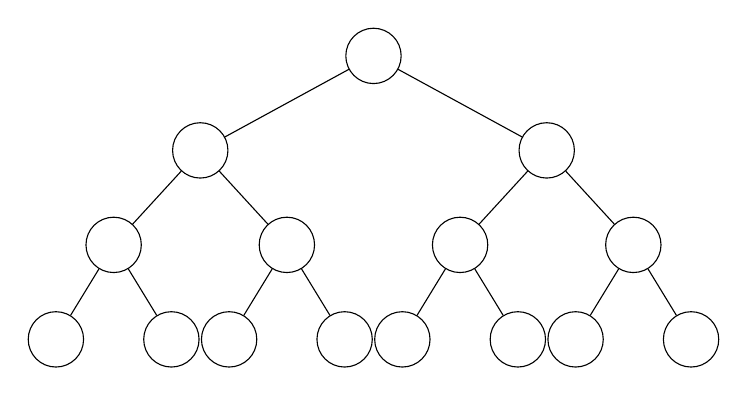
\begin{tikzpicture}[level/.style={sibling distance=55mm/#1},minimum size=25pt,scale=0.8,
    every node/.style={transform shape}]
        \node[circle,draw](z){}
        child{node[circle,draw]{}
            child{node[circle,draw]{}
                child{node[circle,draw]{}
                    child[missing]{}
                    child[missing]{}}
                child{node[circle,draw]{}
                    child[missing]{}
                    child[missing]{}}}
            child{node[circle,draw]{}
                child{node[circle,draw]{}
                    child[missing]{}
                    child[missing]{}}
                child{node[circle,draw]{}
                    child[missing]{}
                    child[missing]{}}}}
        child{node[circle,draw]{}
            child{node[circle,draw]{}
                child{node[circle,draw]{}
                    child[missing]{}
                    child[missing]{}}
                child{node[circle,draw]{}
                    child[missing]{}
                    child[missing]{}}}
            child{node[circle,draw]{}
                child{node[circle,draw]{}
                    child[missing]{}
                    child[missing]{}}
                child{node[circle,draw]{}
                    child[missing]{}
                    child[missing]{}}}};
    \end{tikzpicture}
\end{center}
Insert: \underline{\hspace{.8cm}}
\begin{center}
    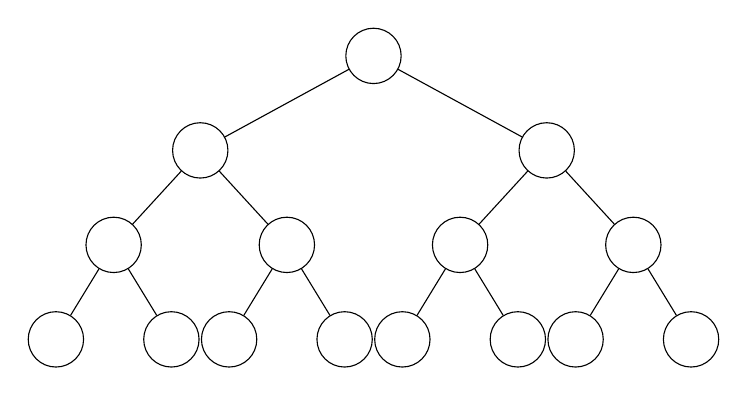
\begin{tikzpicture}[level/.style={sibling distance=55mm/#1},minimum size=25pt,scale=0.8,
    every node/.style={transform shape}]
        \node[circle,draw](z){}
        child{node[circle,draw]{}
            child{node[circle,draw]{}
                child{node[circle,draw]{}
                    child[missing]{}
                    child[missing]{}}
                child{node[circle,draw]{}
                    child[missing]{}
                    child[missing]{}}}
            child{node[circle,draw]{}
                child{node[circle,draw]{}
                    child[missing]{}
                    child[missing]{}}
                child{node[circle,draw]{}
                    child[missing]{}
                    child[missing]{}}}}
        child{node[circle,draw]{}
            child{node[circle,draw]{}
                child{node[circle,draw]{}
                    child[missing]{}
                    child[missing]{}}
                child{node[circle,draw]{}
                    child[missing]{}
                    child[missing]{}}}
            child{node[circle,draw]{}
                child{node[circle,draw]{}
                    child[missing]{}
                    child[missing]{}}
                child{node[circle,draw]{}
                    child[missing]{}
                    child[missing]{}}}};
    \end{tikzpicture}
\end{center}
Insert: \underline{\hspace{.8cm}}
\begin{center}
    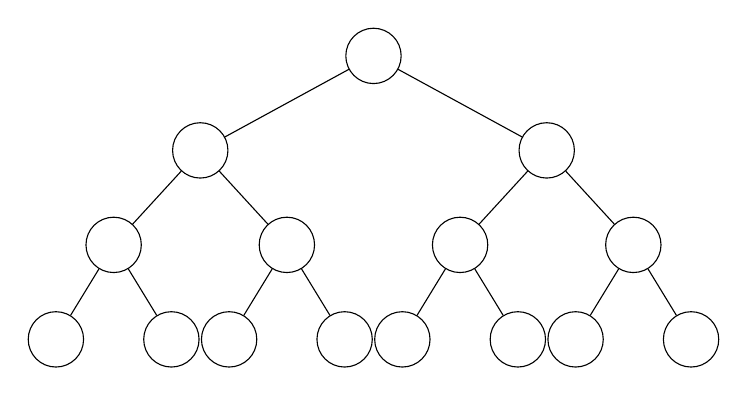
\begin{tikzpicture}[level/.style={sibling distance=55mm/#1},minimum size=25pt,scale=0.8,
    every node/.style={transform shape}]
        \node[circle,draw](z){}
        child{node[circle,draw]{}
            child{node[circle,draw]{}
                child{node[circle,draw]{}
                    child[missing]{}
                    child[missing]{}}
                child{node[circle,draw]{}
                    child[missing]{}
                    child[missing]{}}}
            child{node[circle,draw]{}
                child{node[circle,draw]{}
                    child[missing]{}
                    child[missing]{}}
                child{node[circle,draw]{}
                    child[missing]{}
                    child[missing]{}}}}
        child{node[circle,draw]{}
            child{node[circle,draw]{}
                child{node[circle,draw]{}
                    child[missing]{}
                    child[missing]{}}
                child{node[circle,draw]{}
                    child[missing]{}
                    child[missing]{}}}
            child{node[circle,draw]{}
                child{node[circle,draw]{}
                    child[missing]{}
                    child[missing]{}}
                child{node[circle,draw]{}
                    child[missing]{}
                    child[missing]{}}}};
    \end{tikzpicture}
\end{center}
b) Now perform the known delete$MINMAX$ operation and its sift-operations 5 times
\begin{center}
    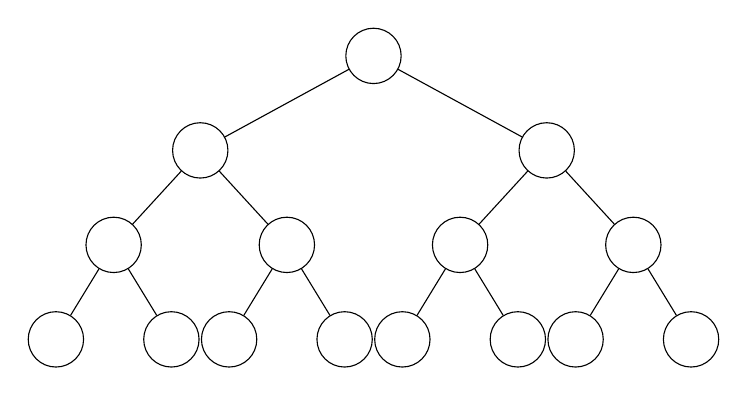
\begin{tikzpicture}[level/.style={sibling distance=55mm/#1},minimum size=25pt,scale=0.8,
    every node/.style={transform shape}]
        \node[circle,draw](z){}
        child{node[circle,draw]{}
            child{node[circle,draw]{}
                child{node[circle,draw]{}
                    child[missing]{}
                    child[missing]{}}
                child{node[circle,draw]{}
                    child[missing]{}
                    child[missing]{}}}
            child{node[circle,draw]{}
                child{node[circle,draw]{}
                    child[missing]{}
                    child[missing]{}}
                child{node[circle,draw]{}
                    child[missing]{}
                    child[missing]{}}}}
        child{node[circle,draw]{}
            child{node[circle,draw]{}
                child{node[circle,draw]{}
                    child[missing]{}
                    child[missing]{}}
                child{node[circle,draw]{}
                    child[missing]{}
                    child[missing]{}}}
            child{node[circle,draw]{}
                child{node[circle,draw]{}
                    child[missing]{}
                    child[missing]{}}
                child{node[circle,draw]{}
                    child[missing]{}
                    child[missing]{}}}};
    \end{tikzpicture}
\end{center}
\begin{center}
    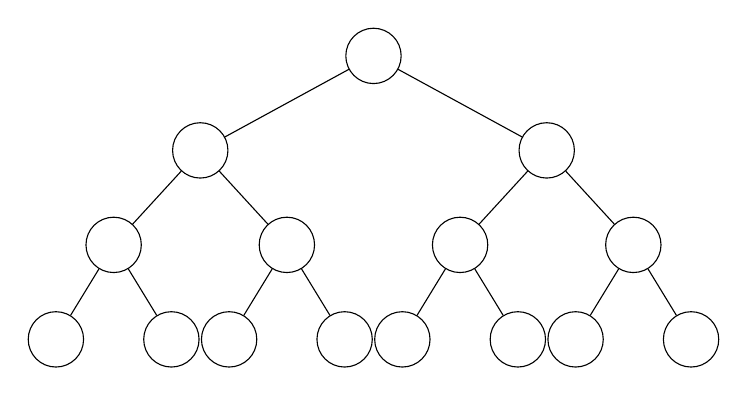
\begin{tikzpicture}[level/.style={sibling distance=55mm/#1},minimum size=25pt,scale=0.8,
    every node/.style={transform shape}]
        \node[circle,draw](z){}
        child{node[circle,draw]{}
            child{node[circle,draw]{}
                child{node[circle,draw]{}
                    child[missing]{}
                    child[missing]{}}
                child{node[circle,draw]{}
                    child[missing]{}
                    child[missing]{}}}
            child{node[circle,draw]{}
                child{node[circle,draw]{}
                    child[missing]{}
                    child[missing]{}}
                child{node[circle,draw]{}
                    child[missing]{}
                    child[missing]{}}}}
        child{node[circle,draw]{}
            child{node[circle,draw]{}
                child{node[circle,draw]{}
                    child[missing]{}
                    child[missing]{}}
                child{node[circle,draw]{}
                    child[missing]{}
                    child[missing]{}}}
            child{node[circle,draw]{}
                child{node[circle,draw]{}
                    child[missing]{}
                    child[missing]{}}
                child{node[circle,draw]{}
                    child[missing]{}
                    child[missing]{}}}};
    \end{tikzpicture}
\end{center}
\begin{center}
    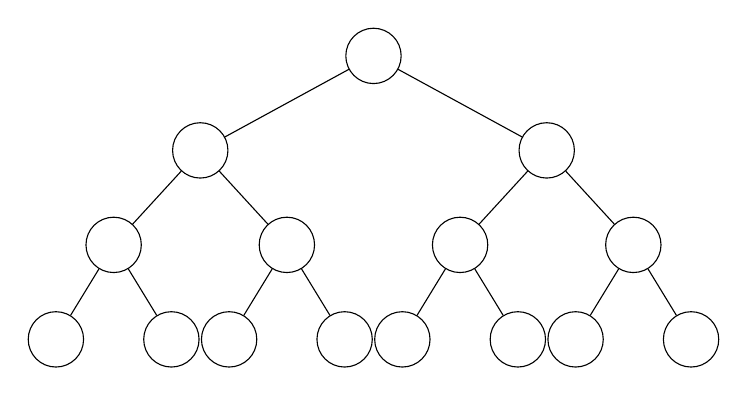
\begin{tikzpicture}[level/.style={sibling distance=55mm/#1},minimum size=25pt,scale=0.8,
    every node/.style={transform shape}]
        \node[circle,draw](z){}
        child{node[circle,draw]{}
            child{node[circle,draw]{}
                child{node[circle,draw]{}
                    child[missing]{}
                    child[missing]{}}
                child{node[circle,draw]{}
                    child[missing]{}
                    child[missing]{}}}
            child{node[circle,draw]{}
                child{node[circle,draw]{}
                    child[missing]{}
                    child[missing]{}}
                child{node[circle,draw]{}
                    child[missing]{}
                    child[missing]{}}}}
        child{node[circle,draw]{}
            child{node[circle,draw]{}
                child{node[circle,draw]{}
                    child[missing]{}
                    child[missing]{}}
                child{node[circle,draw]{}
                    child[missing]{}
                    child[missing]{}}}
            child{node[circle,draw]{}
                child{node[circle,draw]{}
                    child[missing]{}
                    child[missing]{}}
                child{node[circle,draw]{}
                    child[missing]{}
                    child[missing]{}}}};
    \end{tikzpicture}
\end{center}
\begin{center}
    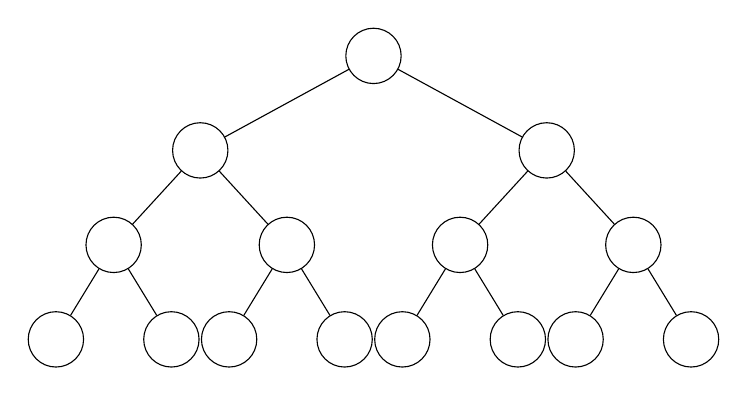
\begin{tikzpicture}[level/.style={sibling distance=55mm/#1},minimum size=25pt,scale=0.8,
    every node/.style={transform shape}]
        \node[circle,draw](z){}
        child{node[circle,draw]{}
            child{node[circle,draw]{}
                child{node[circle,draw]{}
                    child[missing]{}
                    child[missing]{}}
                child{node[circle,draw]{}
                    child[missing]{}
                    child[missing]{}}}
            child{node[circle,draw]{}
                child{node[circle,draw]{}
                    child[missing]{}
                    child[missing]{}}
                child{node[circle,draw]{}
                    child[missing]{}
                    child[missing]{}}}}
        child{node[circle,draw]{}
            child{node[circle,draw]{}
                child{node[circle,draw]{}
                    child[missing]{}
                    child[missing]{}}
                child{node[circle,draw]{}
                    child[missing]{}
                    child[missing]{}}}
            child{node[circle,draw]{}
                child{node[circle,draw]{}
                    child[missing]{}
                    child[missing]{}}
                child{node[circle,draw]{}
                    child[missing]{}
                    child[missing]{}}}};
    \end{tikzpicture}
\end{center}
\begin{center}
    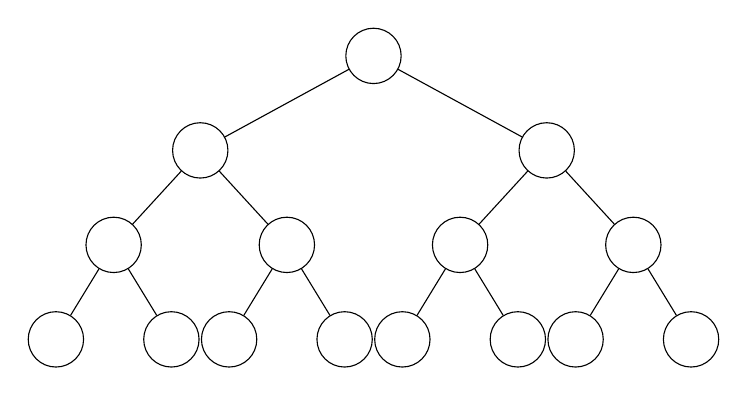
\begin{tikzpicture}[level/.style={sibling distance=55mm/#1},minimum size=25pt,scale=0.8,
    every node/.style={transform shape}]
        \node[circle,draw](z){}
        child{node[circle,draw]{}
            child{node[circle,draw]{}
                child{node[circle,draw]{}
                    child[missing]{}
                    child[missing]{}}
                child{node[circle,draw]{}
                    child[missing]{}
                    child[missing]{}}}
            child{node[circle,draw]{}
                child{node[circle,draw]{}
                    child[missing]{}
                    child[missing]{}}
                child{node[circle,draw]{}
                    child[missing]{}
                    child[missing]{}}}}
        child{node[circle,draw]{}
            child{node[circle,draw]{}
                child{node[circle,draw]{}
                    child[missing]{}
                    child[missing]{}}
                child{node[circle,draw]{}
                    child[missing]{}
                    child[missing]{}}}
            child{node[circle,draw]{}
                child{node[circle,draw]{}
                    child[missing]{}
                    child[missing]{}}
                child{node[circle,draw]{}
                    child[missing]{}
                    child[missing]{}}}};
    \end{tikzpicture}
\end{center}
